\newpage
\section{Critical Design}
\label{sec:critical_design}
%
This section describes in more detail the \ac{EPS} design. A simple block diagram of the \ac{EPS} design is shown in Figure \ref{fig:EPS_diagram_simple}.

\begin{figure}[H]
\centering
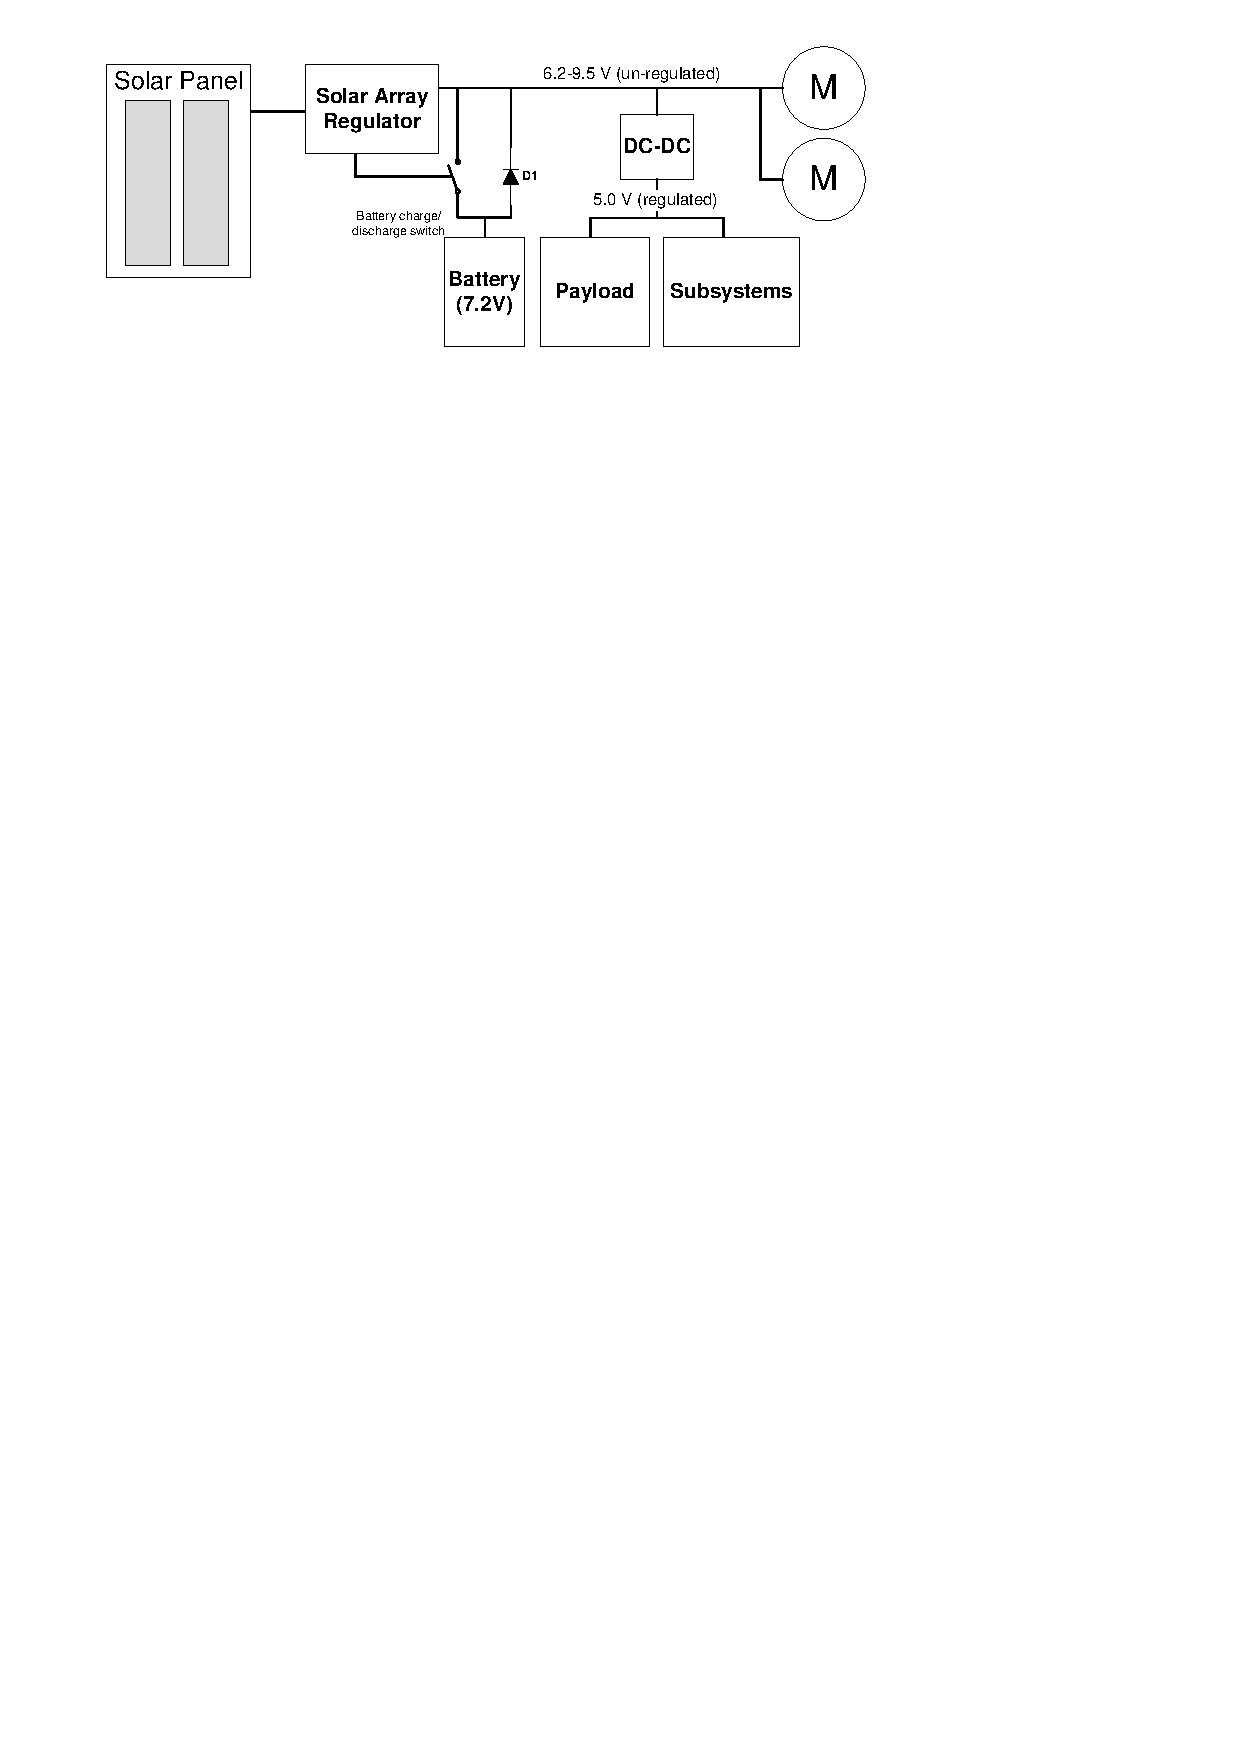
\includegraphics[width=\textwidth]{figures/fig_PDR_EPSdiagram}
\caption{\ac{EPS} simple blockdiagram}
\label{fig:EPS_diagram_simple}
\end{figure}
%
%
\subsection{Solar Array Design}
%Bypass diodes on SA to mitegate shadowing problems
%Cross-strapping of solar cells?
%\subsubsection*{Solar Array Shading}
%Bypass diodes can be used to partly mitigate this issue as well as using \ac{MPPT}. Otherwise it could be necessary to ensure that the airship structure cannot cast shadows on the panels and that the airship only fly above or away from landscape objects.
As was mentioned in section \ref{sec:changes_pdr_to_cdr}, a new solar cell has been selected. This solar cell is shown in Figure \ref{fig:solar_cell} and Table \ref{tab:solar_cell_spec} lists the important specifications for this cell.
%
\begin{figure}[H]
\centering
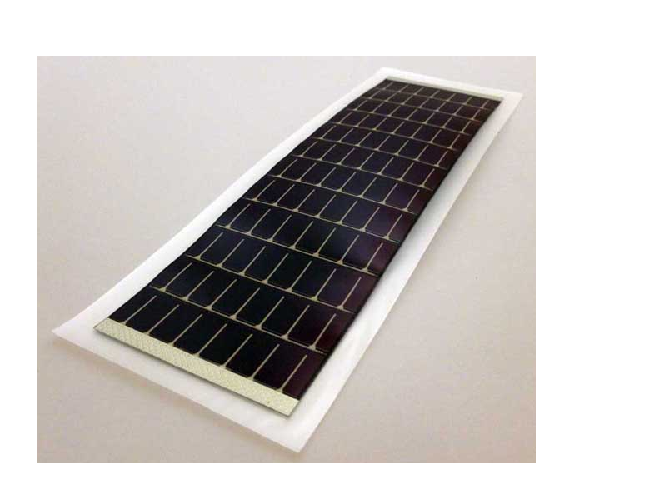
\includegraphics[width=0.3\textwidth]{figures/SolarCell_RC7-2_Powerfilm}
\caption{Chosen solar cell}
\label{fig:solar_cell}
\end{figure}
%
\begin{table}[H]
\centering
\caption{Specifications of chosen solar cell}
\label{tab:solar_cell_spec}
\begin{minipage}{\textwidth}
\begin{tabular}{ll}
\hline
Nominal output current & $100\,mA$\\
Nominal output voltage & $7.2V$\\
Nominal output power & $0.72\,W$\\
Dimensions & $270\,mm\:\times\:90\,mm\:\times\:0.2\,mm$\\
Weight & $7.6\,g$\\
No. of required cells $100$\footnote{\cite{avnetexpress} offers good discount for +100 units order}\\
Total solar panel area & $2.43\,m^2$ (assuming $100\,\%$ fill factor)\\
\hline
\end{tabular}\par
\vspace{-0.75\skip\footins}
\renewcommand{\footnoterule}{}
\end{minipage}
\end{table}
%
%
The solar panels will be configured with two series-connected solar cells thus having an output voltage of: 
%
\begin{equation}
V_{panel,out}=14.4\,V
\end{equation}
%
%
\subsection{Battery Design}
%
Two Panasonic PA-L60.K02 \cite{panasonic} Li-ion batteries are used. The battery has the following important specifications:
%
\begin{table}[H]
\centering
\caption{Specification of chosen battery}
\label{tab:proposed_battery}
\begin{tabular}{ll}
\hline
Chemistry & Li-ion\\
Nominal voltage & $3.6\,V$\\
Capacity & $1.03\,Ah$ / $3.61\,Wh$\\
Weight & $25\,g$\\
Dimensions & $56\,mm\:\times\:34.2\,mm\:\times\:5.8\,mm$\\
Maximum charge current & $970\,mA$\\
Maximum discharge current (continuous) & $1.455\,A$\\
\hline
\end{tabular}
\end{table}
%
%
\subparagraph*{Future Recommendations}
%
The chosen type of Li-ion battery supports only a relative low charge- and discharge rate of about $1\,C$. For bigger battery capacity and higher loads, it is recommended to use a battery like \cite{rcflight_battery} which provides much higher discharge rates ($>20\,C$) and also cheaper price per Wh. Only disadvantage  is a mass increase of around $15-25\%$.
%
\subsubsection{Battery Charge Regulator}
%
From the battery datasheet, maximum charge current is $I_{REG}=970\,mA$. From the \ac{BCR} datasheet, the minimum current sense resistor value is calculated as
%
\begin{equation}
\begin{split}
R_{sense}=&\dfrac{V_{FCS}}{I_{REG}}\\
R_{sense}=&\dfrac{120\,mV}{970\,mA}=123\,m\Omega
\end{split}
\end{equation}
%
The required thermal rating of the pass transistor is calculated as
%
\begin{equation}
P_{max}=(V_{in,max}-V_{bat,min})\cdot I_{charge}=(9.5\,V-5.5\,V)\cdot 970\,mA=3.88\,W
\end{equation}
%
\subsubsection{Battery Temperature Monitoring}
%
The \ac{BCR} chip includes a temperature monitoring feature. The battery is rated, in charge-mode, to temperature in the interval $10-45^{\circ}C$. The maximum allowed temperature is set slightly lower to $40^{\circ}C$. The Li-ion battery has a build-in \ac{NTC} thermistor with $B=3980\,K$ and $R_{25}=10k\,\Omega$. The required restance values of the temperature control resistors are determined from the \ac{BCR} chip datasheet as 
%
\begin{equation}
\begin{split}
R_{cold}&=R_{25}e^{B(\dfrac{1}{T}-\dfrac{1}{T_0}}=10\,k\Omega e^{3980\,K(\dfrac{1}{283	\,K}-\dfrac{1}{298\,K})}=20.3\,k\Omega\\
R_{hot}&=10\,k\Omega e^{3980\,K(\dfrac{1}{313	\,K}-\dfrac{1}{298\,K})}=5.3\,k\Omega\\
R_{T1}&=2\dfrac{R_{cold}R_{hot}}{R_{cold}-R_{hot}}=14.2\,k\Omega\\
R_{T2}&=2\dfrac{R_{cold}R_{hot}}{R_{cold}-3R_{hot}}=47.8\,k\Omega
\end{split}
\end{equation}

%
\subsubsection{Battery Discharge Current Limiter}
%
The battery in \cite{panasonic} has a maximum discharge rate current of $I_{discharge}=1.455\,A$. A discharge current limiter circuit has been added as shown in Figure \ref{fig:EPS_diagram_detailed}. In normal conditions, the MOSFET is off making the base pin of the \ac{PNP} \ac{BJT} low and hence the BJT is fully conducting. When the current through the sense resistor increases, the voltage on the PNP MOSFET gate starts to drop and at the current limit point begins to conduct. When this happens, the base of the BJT is pulled up on the device starts to limit the current.

The selected MOSFET has a typical gate threshold voltage of $V_{Gth}=550\,mV$. The chosen \ac{BJT} has a typical collector-emitter voltage drop of $V_{CE}=120\,mV$. The required current sense resistor is then calculated as 
%
\begin{equation}
\begin{split}
V_{sense}&=V_{Gth}-V_{CE}=550\,mV-120\,mV=430\,mV \Rightarrow\\
R_{sense}&=\dfrac{V_{sense}}{I_{discharge}}=\dfrac{430\,mV}{1.455\,A}=295\,m\Omega
\end{split}
\end{equation}
%
The exact required resistance must be determined by testing the precise parameters of the discrete components. The $500\,\Omega$ resistor value is chosen as a compromise between the power loss from current drawn in current limitation mode $P_{loss}\approx V_{bat}^2/R_2$ and the requirement that the resistor must allow about $10\,mA$ (base current) to be drawn at the lowest voltage across the resistor which is about $5\,V$.
%
%
%
\subsection{Maximum Power Point Tracking Regulator}
%Which design concepts are considered? - What are the advantages/disadvantages for each concept?
%Decide on MPPT algorithm (using analog circuits?)
%DC-DC regulator topology (Buck, Boost, Buck-Boost etc.)
%
In \cite{PDR} it was decided to use a \ac{MPPTU} for the \ac{APR} due to its high efficiency and robustness to changing environmental constraints.

In first step, only the DC-DC converter will be implemented. When time and resources allows the \ac{MPPT} part will be added.
A simple buck DC-DC converter topology is used, comprising a transistor, free-wheel diode, inductor and output capacitor. 
When the full \ac{MPPTU} is implemented, it will operate in three different operation regions:
%
\begin{itemize}
\item Battery discharge {MPPT} - when the solar array input power is insufficient to cover the load power demand, the battery is slowly discharged in order to maintain the output voltage.
\item Battery charge {MPPT} - when the solar array input is greater than the load power, the excessive power is used to recharge the battery.
\item Input power limitation - when the battery is fully charged, the regulator will operate the solar array at a non-optimal voltage, thus limiting the input power to keep the output voltage constant. The extra potential input power is dissipated as heat externally on the solar arrays.
\end{itemize}
%
\begin{figure}[H]
\centering
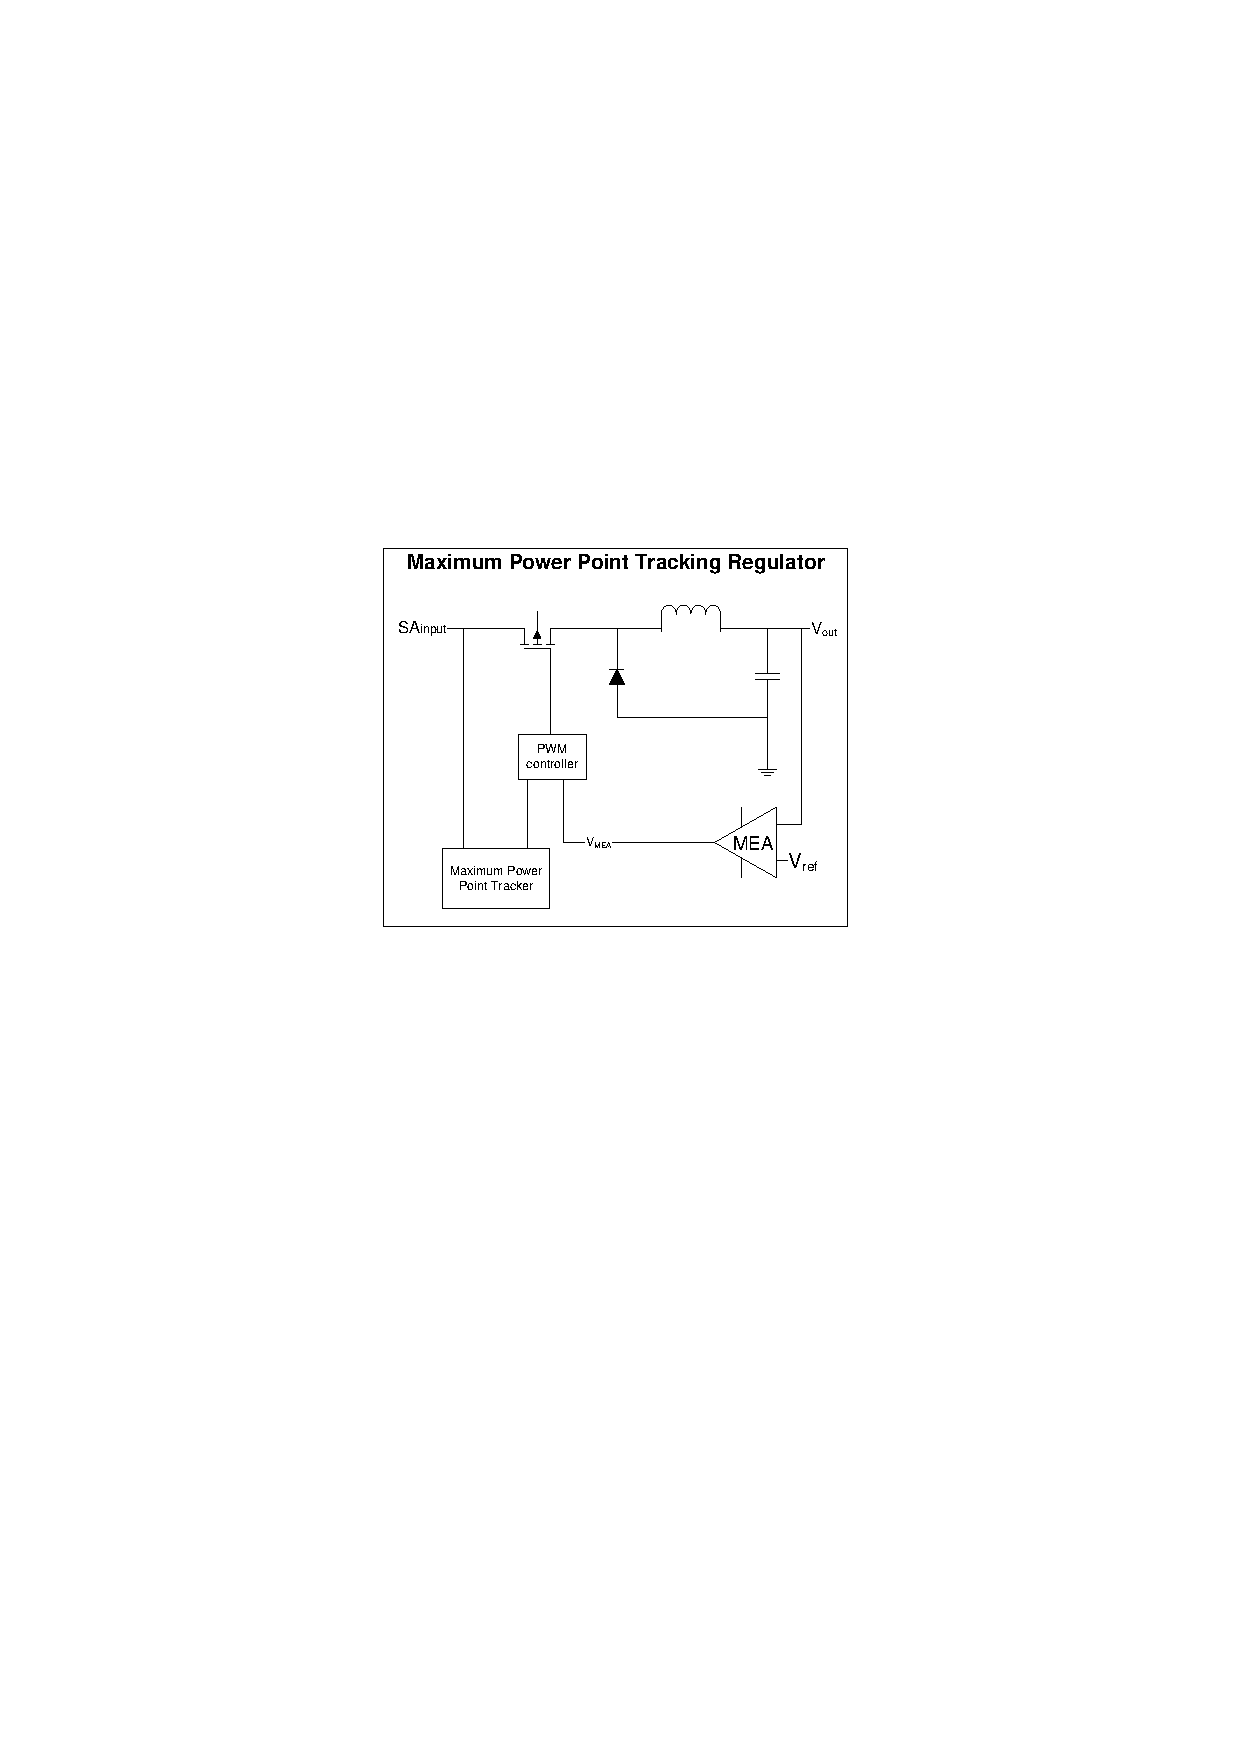
\includegraphics[scale=1]{figures/fig_PDR_MPPTdiagram}
\caption{\ac{MPPT} regulator diagram}
\label{fig:MPPT_regulator}
\end{figure}
%


\subsubsection{Mainbus Under Voltage Protection}
%
The power from battery and solar cells is limited. It is thus possible that the motors will try to draw more current than what can be delivered. If this happens, the output capacitor of the \ac{APR} will quickly discharge and the main output voltage drops out. To prevent this situation, an \ac{UVP} circuit is added. This is implemented using an $STN888$ PNP \ac{BJT} along with two resistors, $R3$ and $R4$ as shown in Figure \ref{fig:EPS_diagram_detailed}. When the main output voltage is around $6.2\,V$ the Base-Emitter voltage drop is close to $1.2\,V$ and the \ac{BJT} is fully conducting and effectively works as a short circuit. If the output voltage drops significantly below $6.2\,V$ the \ac{BJT} will begin to decrease the output current until the output voltage stabilizes. The current gain of $STN888$ is about $100$, hence to allow an maximum output current of $10\,A$, the resistors $R3$ and $R4$ must be designed to pass $100\,mA$ at $6.2\,V$ output voltage. To minimize efficiency it is important that the forward voltage drop of the \ac{BJT} is kept as low as possible.

\subparagraph*{Further Recommendations}
%
It is hard to find suitable \acp{BJT} rated for much more than $5\,A$. If the power output is increased in future designs, it is suggested to either parallel connect several \acp{BJT} however this might cause issues with thermal runaway. Alternatively high current \acp{IGBT} can be used, however they have higher forward voltage drops and thus they are more suitable for a design with a higher output voltage.


%
\subsection{Complete EPS Diagram}
%
The complete \ac{EPS} diagram is shown in Figure \ref{fig:EPS_diagram_detailed}. For providing the $5\,V$ regulated voltage to the payloads, \ac{COTS} DC-DC regulator(s) are used. The battery charging/discharging is controlled by the \ac{SAR}.
%
\begin{sidewaysfigure}
\centering
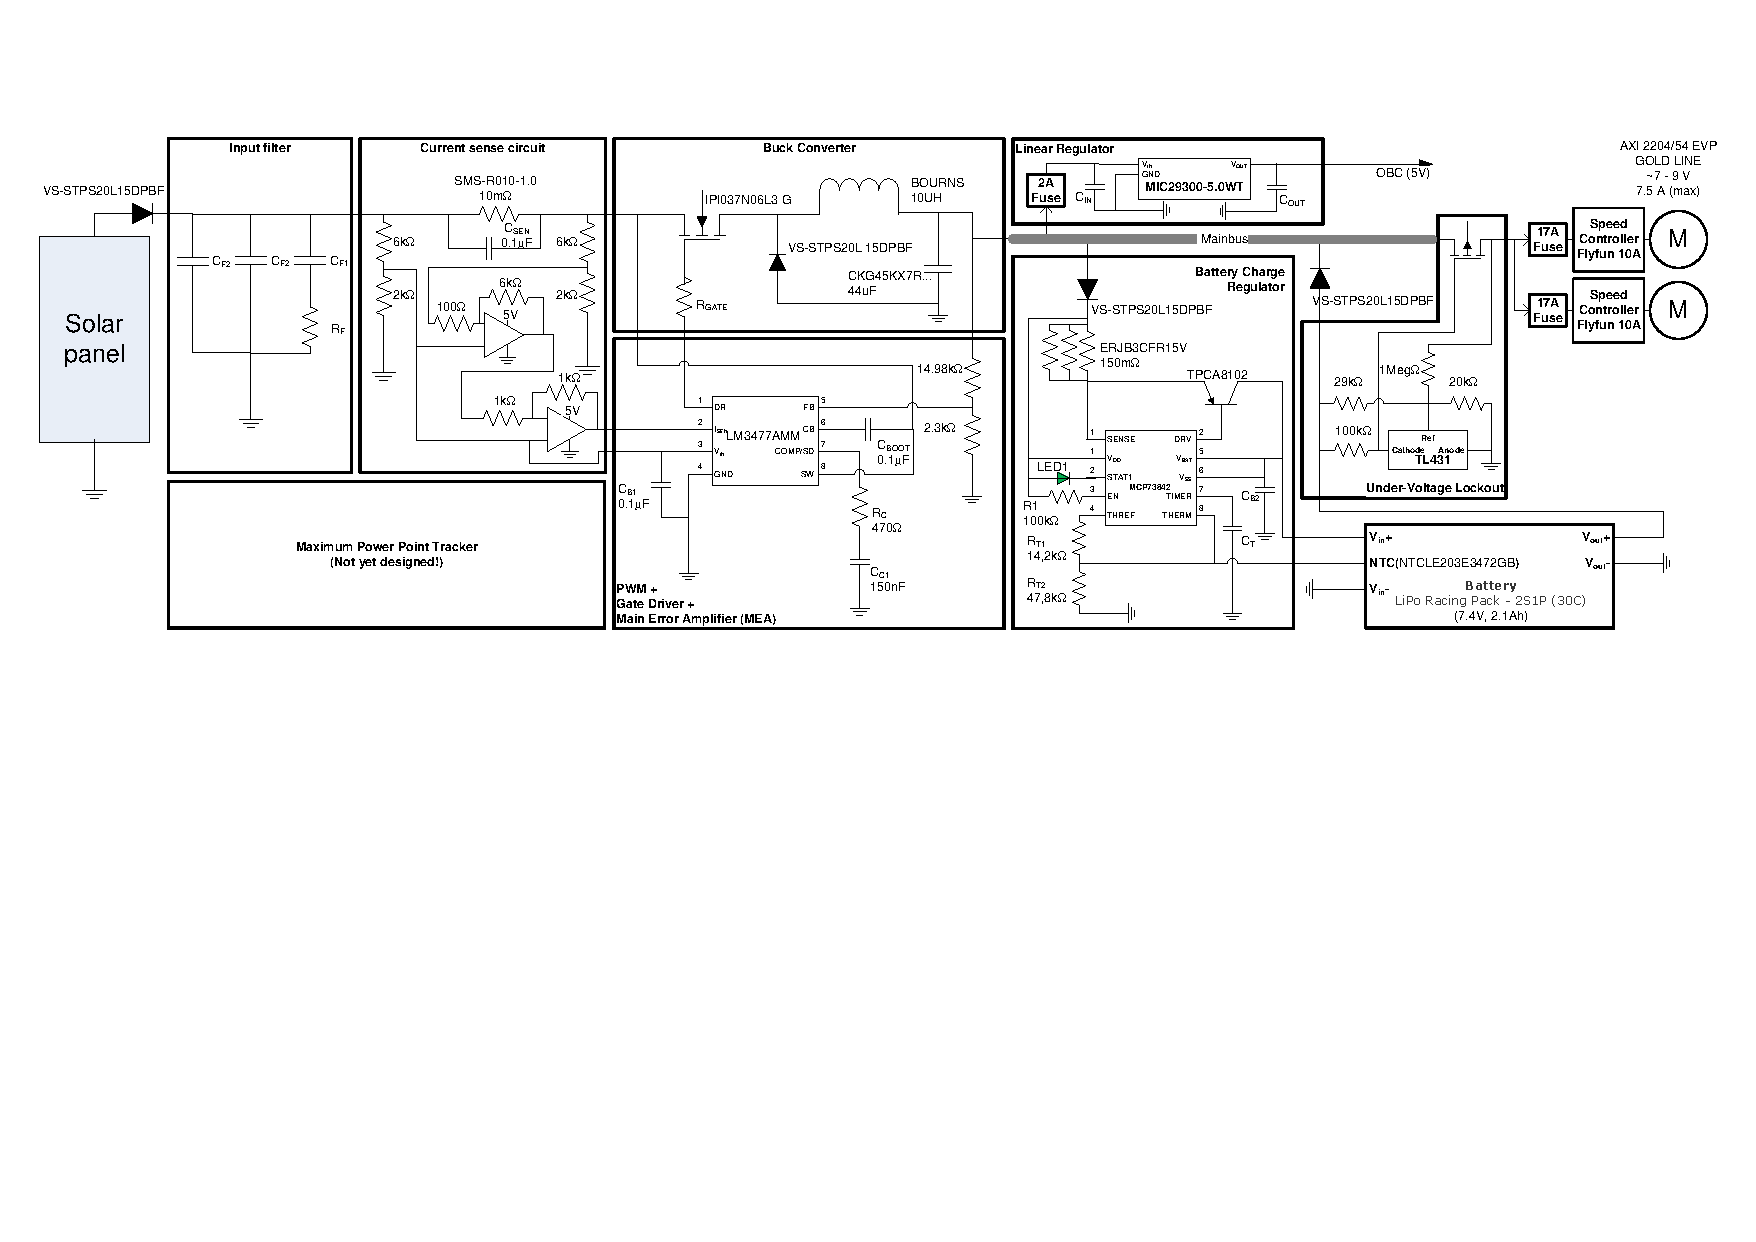
\includegraphics[scale=0.8]{figures/fig_CDR_EPSdiagram_detailed}
\caption{\ac{EPS} detailed block diagram diagram}
\label{fig:EPS_diagram_detailed}
\end{sidewaysfigure}

%
\subsection{External Interfaces}
%
The interfaces of the \ac{EPS} external are listed in table \ref{tab:external_interfaces}.
%
\begin{table}[H]
\centering
\caption{External interfaces}
\label{tab:external_interfaces}
\begin{tabular}{m{0.35\textwidth}m{0.55\textwidth}}
\hline
\textbf{External interface} & \textbf{Implementation}\\
\hline
Solar cells mounting & \ac{PSA}\\[2mm]
DC-DC regulators & Mounted on PCB which sits in system housing. Thermal contact points should be included, to remove internal heat dissipation.\\[2mm]
Battery telemetry & Analog signals to Microcontroller\\[2mm]
Mounting of batteries & \ac{TBD}\\
%Output voltage control(reference voltage setpoint) & Analog signal from Microcontroller\\[2mm]
Supply voltages & $6.0-9.2\,V$ (unregulated) and $5.0\,V$(regulated)\\[2mm]
\hline
\end{tabular}
\end{table}
%
%
\subsection{Telemetry and Telecommands}
%What telemetries/telecommands are required/useful for the subsystem? – What data rates/sizes are required?
%
The required/recommended telemetry and telecommands, \ac{EPS} , are listed in table \ref{tab:Telemetry_Telecommands}.
%
\begin{table}[H]
\centering
\caption{Telemetry and telecommands}
\label{tab:Telemetry_Telecommands}
\begin{tabular}{|l|l|l|}
\hline
\textbf{Telemetry} & \textbf{Data rate/frequency} & \textbf{Data size} \\
\hline
Battery voltage & Every 30 sec & 2 bytes\\
\hline
Battery temperature & Every 5 sec & 2 bytes\\
\hline
%Solar array temperature & Every 30 sec & 1 byte\\
%\hline
%Solar array voltage & Every 1 sec(MPPT performance) & 2 bytes\\
%\hline
%Solar array current & Every 1 sec(MPPT performance) & 2 bytes\\
%\hline
\end{tabular}
\end{table}